\chapter{Contexto tecnológico}
\label{chap:contexto}

\section{Python y el problema del GIL}
\label{sec:python-paralelo}

Python gestiona la memoria mediante contadores de referencia. Para evitar
condiciones de carrera en esos contadores cuando múltiples hilos acceden al
mismo objeto, el intérprete CPython mantiene el GIL, un mutex global que solo
permite a un hilo ejecutar bytecode Python en cada instante. La consecuencia
práctica es que los programas Python multihilo no pueden aprovechar múltiples
núcleos para trabajo intensivo en el intérprete, incluso en sistemas con
decenas de cores disponibles.

La restricción no impide toda forma de paralelismo. Extensiones nativas como
NumPy~\cite{NumPy2020} liberan el GIL durante operaciones vectoriales,
compiladores como Numba~\cite{Numba2015} generan código máquina para funciones
numéricas, y bibliotecas como mpi4py~\cite{mpi4py2011} o Dask~\cite{Dask2015}
distribuyen el trabajo mediante procesos. El propio módulo
\texttt{multiprocessing} evita el problema con procesos independientes y memoria
privada. Sin embargo, ninguna de esas vías permite expresar paralelismo de
memoria compartida al nivel del código Python, con el modelo de hilos y
directivas que caracteriza a OpenMP.

Las versiones \emph{free-threaded} de Python eliminan el GIL. Disponibles de
forma experimental desde Python~3.13t~\cite{PEP703}, sustituyen los contadores
de referencia por mecanismos atómicos y biased locking. Esto añade un pequeño
sobrecoste en código monohilo, pero hace posible la ejecución paralela real con
hilos Python. Este TFM utiliza Python~3.15.0b1t como entorno principal y compara
sus resultados con Python~3.13.13t y Python~3.14.4t, compilados también con el
GIL desactivado.


\section{OMP4Py}
\label{sec:omp4py}

OMP4Py es una implementación del modelo de programación OpenMP para
Python~\cite{PineiroOMP4PyFGCS2026,PineiroOMP4PyCGO2026}. Su objetivo es
permitir que el programador exprese regiones paralelas, distribución de
iteraciones y sincronización mediante directivas integradas en código Python,
con una sintaxis análoga a la de OpenMP en C, C++ o
Fortran~\cite{OpenMPSpec,DagumMenon1998}.

Las directivas se expresan como gestores de contexto:

\begin{verbatim}
with omp("parallel for"):
    for i in range(n):
        ...
\end{verbatim}

La biblioteca ofrece cuatro modos de ejecución, seleccionables en tiempo de
ejecución mediante el argumento \texttt{-m}:

\begin{center}
\begin{tabular}{c|l|l}
Modo & Nombre & Descripción \\
\hline
0 & puro      & Runtime puro de OMP4Py en Python; kernels sin compilar. \\
1 & híbrido   & Runtime nativo (Cython) si está disponible; kernels sin compilar. \\
2 & compilado & Kernels compilados a Cython; tipos inferidos. \\
3 & compilado tipado & Cython con anotaciones de tipo explícitas y memoryviews. \\
\end{tabular}
\end{center}

En los cuatro modos, las directivas se transforman mediante el árbol sintáctico
abstracto (AST) del módulo \texttt{ast} de Python y el paralelismo se ejecuta
con hilos reales de la API \texttt{threading}, de modo que en
Python~\emph{free-threaded} pueden aprovechar múltiples núcleos. La diferencia
entre modos está en qué partes del código se compilan
(Figura~\ref{fig:contexto-pipeline}). En los modos~0 y~1 los kernels del
usuario no se compilan. El modo~0 fuerza el runtime puro de OMP4Py, cuyas
primitivas de distribución de trabajo y sincronización están implementadas en
Python, y actúa como línea base funcional. El modo~1 usa el runtime por
defecto, que emplea la implementación nativa del propio runtime, compilada con
Cython, cuando está disponible. Los modos~2 y~3 compilan además los kernels del
usuario a C mediante Cython~\cite{Cython2011}. La
diferencia entre ellos es que el modo~3 permite anotar variables con tipos
Cython (\texttt{cython.double}, \texttt{cython.int}, memoryviews) para eliminar
la indirección de los objetos Python en los bucles numéricos.

\begin{figure}[htbp]
\centering
\resizebox{\textwidth}{!}{%
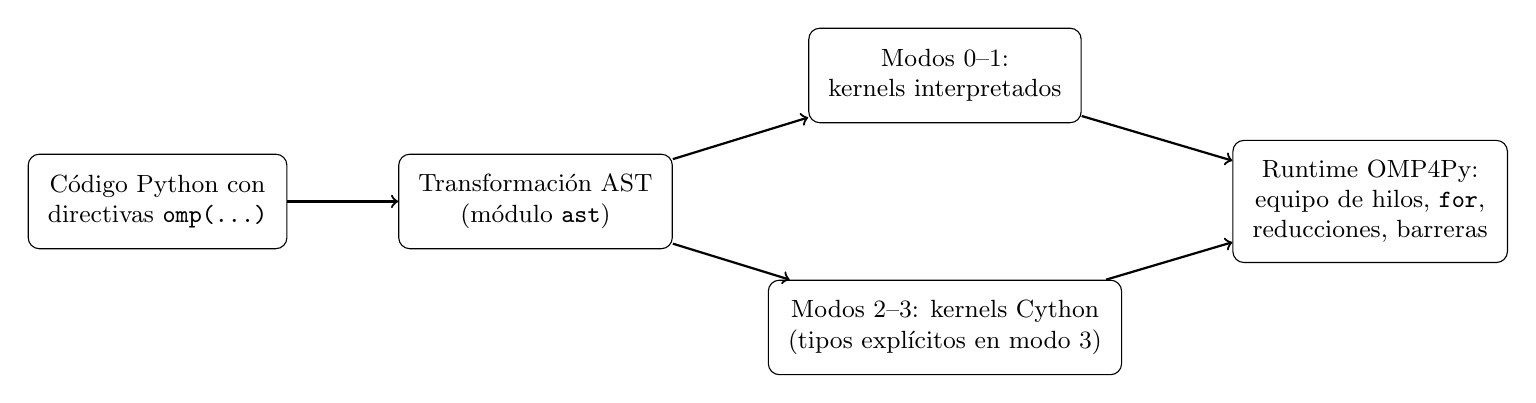
\begin{tikzpicture}[
  caja/.style={draw, rounded corners, align=center, minimum height=12mm,
               inner sep=2.5mm, font=\small},
  flecha/.style={->, thick}
]
  \node[caja] (src) at (0,0) {Código Python con\\directivas \texttt{omp(...)}};
  \node[caja] (ast) at (4.8,0) {Transformación AST\\(módulo \texttt{ast})};
  \node[caja] (pure) at (10.0,1.6) {Modos 0--1:\\kernels interpretados};
  \node[caja] (cy)  at (10.0,-1.6) {Modos 2--3: kernels Cython\\(tipos explícitos en modo 3)};
  \node[caja] (rt)  at (15.4,0) {Runtime OMP4Py:\\equipo de hilos, \texttt{for},\\reducciones, barreras};
  \draw[flecha] (src) -- (ast);
  \draw[flecha] (ast) -- (pure);
  \draw[flecha] (ast) -- (cy);
  \draw[flecha] (pure) -- (rt);
  \draw[flecha] (cy) -- (rt);
\end{tikzpicture}
}
\caption{Flujo de ejecución de un programa OMP4Py. Las directivas se procesan
mediante transformación AST en todos los modos. El modo determina si los
kernels del usuario se compilan con Cython y qué implementación del runtime
ejecuta la distribución de trabajo y la sincronización.}
\label{fig:contexto-pipeline}
\end{figure}

La compilación en los modos~2 y~3 se realiza en tiempo de ejecución, antes del
primer uso de cada kernel. Los kernels compilados se almacenan en caché para
reutilizarlos en ejecuciones posteriores.

La diversidad de modos permite aislar tres factores de rendimiento: el coste del
runtime Python frente al runtime compilado, el impacto del tipado Cython sobre
los bucles numéricos y la ganancia real del paralelismo entre hilos.


\section{NAS Parallel Benchmarks}
\label{sec:nas}

Los NAS Parallel Benchmarks (NPB) son un conjunto de benchmarks desarrollado
por NASA para evaluar sistemas paralelos~\cite{NPB1994}. Cada benchmark
implementa un núcleo computacional representativo de aplicaciones de
simulación numérica.

\begin{itemize}
  \item \textbf{EP} (\emph{Embarrassingly Parallel}): generación de pares
        aleatorios gaussianos mediante el método de Box-Muller. El trabajo
        útil es embarazosamente paralelo. La única sincronización es una
        reducción global al final.
  \item \textbf{CG} (\emph{Conjugate Gradient}): estimación del menor
        autovalor de una matriz dispersa irregular mediante gradiente conjugado.
        Requiere productos matriz-vector, actualizaciones de vectores y
        reducciones escalares en cada iteración.
  \item \textbf{IS} (\emph{Integer Sort}): ordenación entera mediante un
        algoritmo de counting sort por cubos. Exige paralelismo en histogramas,
        offsets y ordenación local con semántica estricta.
  \item \textbf{MG} (\emph{Multi-Grid}): resolución aproximada de la ecuación
        de Poisson 3D mediante el método multigrid. Opera sobre mallas en varios
        niveles de resolución con operaciones de restricción, prolongación e
        interpolación.
  \item \textbf{FT} (\emph{Fourier Transform}): solución de una EDP mediante
        transformadas de Fourier 3D complejas. El kernel principal es una FFT
        aplicada sucesivamente a cada dimensión de un array tridimensional de
        números complejos.
\end{itemize}

Cada benchmark define varias clases de problema (S, W, A, B, C, D), asociadas a
tamaños de malla o números de iteraciones crecientes. Esta escala permite
estudiar el comportamiento de OMP4Py en cargas de distinta granularidad sin
cambiar de benchmark.

Los NPB incluyen rutinas de verificación internas que comprueban la exactitud
numérica del resultado. Esa verificación es la única condición de aceptación
utilizada en este trabajo. Una adaptación que ejecute más rápido pero no
verifique correctamente se rechaza.


\section{Trabajo relacionado}
\label{sec:trabajo-relacionado}

El paralelismo en Python se ha abordado tradicionalmente por vías que evitan el
GIL en lugar de eliminarlo. Las extensiones nativas como NumPy~\cite{NumPy2020}
liberan el GIL durante operaciones vectoriales, y compiladores como
Numba~\cite{Numba2015} o Cython~\cite{Cython2011} generan código máquina para
funciones numéricas. En todos los casos el modelo de programación paralela queda
oculto en la capa nativa y no se expresa al nivel del código Python. La
excepción más próxima a OMP4Py es PyOMP~\cite{PyOMP2021}, que añade directivas
OpenMP a funciones compiladas con Numba. Su alcance queda, sin embargo,
restringido al subconjunto del lenguaje que Numba puede compilar, mientras que
OMP4Py opera sobre código Python estándar y delega en Cython la compilación
opcional de los kernels. El
paralelismo de procesos (\texttt{multiprocessing}, mpi4py~\cite{mpi4py2011} o
Dask~\cite{Dask2015}) escala a múltiples nodos, pero con memoria privada y un
coste de comunicación que no corresponde al modelo de memoria compartida de
OpenMP~\cite{OpenMPSpec,DagumMenon1998}.

La eliminación del GIL en las versiones \emph{free-threaded}~\cite{PEP703} abre
una vía distinta: ejecutar hilos Python reales sobre memoria compartida.
OMP4Py~\cite{PineiroOMP4PyFGCS2026,PineiroOMP4PyCGO2026} se sitúa en esa vía al
trasladar el modelo de directivas de OpenMP al código Python. Este trabajo se
diferencia de los estudios que presentan la propia biblioteca en que su objeto
no es OMP4Py en sí, sino su evaluación sobre aplicaciones completas y a lo largo
de varias versiones del intérprete.

Como cargas de trabajo se emplean los NAS Parallel Benchmarks~\cite{NPB1994},
ampliamente utilizados para evaluar sistemas paralelos. Existen portados previos
de los NPB a Python a partir de las versiones seriales en C++~\cite{NPBPython},
que sirven de base serial para la adaptación descrita en el
Capítulo~\ref{chap:adaptacion-nas}. Hasta donde alcanza este trabajo, la
evaluación de OMP4Py sobre kernels NPB completos, con sus cuatro modos de
ejecución y la comparación entre versiones \emph{free-threaded} de Python, no se
había abordado de forma sistemática.
